\documentclass{article}
\usepackage[utf8]{inputenc}
\usepackage{amsfonts}
\usepackage{tikz}
\usepackage{natbib}
\usepackage{url}
\usepackage{graphicx,amsmath,amsthm,amssymb}
\usepackage{eucal}
\usepackage{color}
\graphicspath{ {images/} }
\newcommand{\vect}[2]{\bigl[\begin{smallmatrix}#1\\#2\end{smallmatrix}\bigr]}
\newcommand{\vectt}[3]{\bigl[\begin{smallmatrix}#1\\#2\\#3\end{smallmatrix}\bigr]}
\newcommand{\Z}{\mathbb{Z}}
\newcommand{\R}{\mathbb{R}}
\newcommand{\C}{\mathbb{C}}
\newcommand{\CP}{\hat{\mathbb{C}}}

\title{A Space of Circle Packing Algorithms}
\author{Connor Riley, Don Sheehy, Kevin Pratt, Kirk Gardner}
\date{February 2016}

\begin{document}
\maketitle
\section{Introduction}
The Circle packing theorem was first discovered by Paul Koebe and then later reintroduced by William Thurston in 1985. As a result, this is a relatively new topic to many mathematicians and Computer Scientists. 
\section{Definitions}
 \subsection{Graphs}
  A \textbf{graph} is an ordered pair $G=(V,E)$ which represents a set of objects where some of these objects are linked. In the denotation $G=(V,E)$, $V$ stands for the vertexes or objects, and $E$ stands for the edges or links. Edges in a graph can be directed or undirected, however, we will focus on undirected edges in our application.

  A component or \textbf{connected component} of a graph is a subgraph in which any two vertices are connected to each other by a path which is connected to no additional vertices in the supergraph.

  A \textbf{loop} is when a vertex has an edge connecting it to itself. \citep{NIST:self-loop}
  
  \begin{figure}[h]
  \centering
	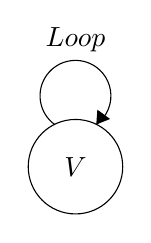
\begin{tikzpicture}[scale=0.2]\tikzstyle{every node}+=[inner sep=0pt]
	  \draw [black] (25.7,-24.2) circle (3);
	  \draw (25.7,-24.2) node {$V$};
      \draw [black] (24.377,-21.52) arc (234:-54:2.25);
      \draw (25.7,-16.95) node [above] {$Loop$};
      \fill [black] (27.02,-21.52) -- (27.9,-21.17) -- (27.09,-20.58);
    \end{tikzpicture}
    \caption{A loop.}
    \label{fig: loop}
  \end{figure}
  
  A graph with multiple edges is one which has two or more edges connect the same two vertices.\\
  
  \begin{figure}[h]
    \centering
	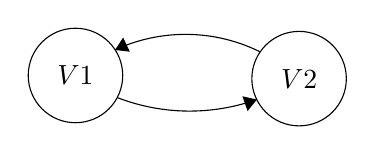
\begin{tikzpicture}[scale=0.2]\tikzstyle{every node}+=[inner sep=0pt]
	  \draw [black] (25.7,-24.2) circle (3);
	  \draw (25.7,-24.2) node {$V1$};
	  \draw [black] (39.9,-24.4) circle (3);
	  \draw (39.9,-24.4) node {$V2$};
	  \draw [black] (37.217,-25.726) arc (-70.44515:-111.16871:12.75);
	  \fill [black] (37.22,-25.73) -- (36.3,-25.52) -- (36.63,-26.46);
	  \draw [black] (28.21,-22.575) arc (114.84766:63.53848:10.656);
	  \fill [black] (28.21,-22.58) -- (29.15,-22.69) -- (28.73,-21.79);
	\end{tikzpicture}
	\caption{A graph with multiple edges.}
      \label{fig: multiple edges}
  \end{figure}

 \subsubsection{Types of Graphs}
  A graph is \textbf{connected} when there is a path between every pair of vertices. 
  In a connected graph every vertex is reachable. A graph with just one vertex is connected~\citep{mathworld:ConnectedGraphs}. A graph is said to be k-connected if there does not exist a set of k-1 vertices whose removal disconnects the graph. Typically we will work with 3-connected graphs - this means that three vertices would have to be removed to disconnect the graph.
  
  A \textbf{simple graph} is an unweighted, undirected graph, containing no loops or multiple edges. 
  A simple graph may either be connected or disconnected~\citep{mathworld:SimpleGraphs}.
  
  A \textbf{planar graph} is one that can be embedded in the plane. 
  In other words, the graph can be drawn on the plane in such a way that its edges intersect only at their endpoints (no edges cross each other)~\citep{mathworld:PlanarGraph}. By $Whitney's$ $Theorem$ if a graph is planar and 3-connected, all the faces of the graph will be the same shape. A Triangulated graph, or triangulation is an example of this property.
  
  A \textbf{triangulation}, also referred to as a \textbf{maximal planar graph}, is a planar graph in which there is no way to add another edge and have the graph continue to be planar. In practice this means that each face is bounded by three edges\citep{mathworld:Triangulation}.
  
  \textbf{Euler's formula} states that if a finite, connected, planar graph is drawn in the plane without any edge intersections, and $v$ is the number of vertices, $e$ is the number of edges and $f$ is the number of faces (including the outer region), then: 
  \begin{equation} 
	v-e+f=2
  \end{equation}
  
  \subsection{Embedding}
  A \textbf{simple arc} is an image of a continuous injective map [0,1] $\rightarrow \Sigma$.\\
  \begin{figure}[h]
      \centering
      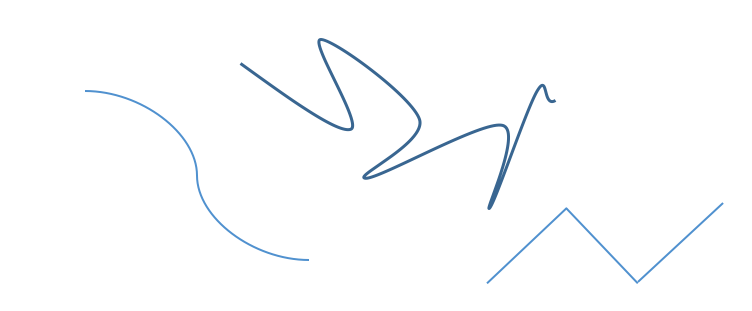
\includegraphics[scale=.3]{simple_arcs}       
      \caption{Three simple arcs.}
      \label{fig: Figure 3}
  \end{figure}\\
  An \textbf{embedding} of a graph $G$ on a surface $\Sigma$ is a representation of $G$ on $\Sigma$ in which points of $\Sigma$ are associated to vertices and simple arcs are associated to edges in such a way that:
  \begin{itemize}
	\item The endpoints of the arc associated to the edge $e$ are the points associated to the end vertices of $e$.
	\item No arcs include points associated with other vertices.
	\item Two arcs never intersect at a point which is interior to either of the arcs.
  \end{itemize}
  This can be stated mathematically as the following: Given edges $e=(u,v)$, the function mapping the vertices to the plane $ \phi :V \rightarrow \R^2$, and the function mapping the edges to the plane $ \rho_e :[0,1] \rightarrow \R^2$, the embedding $= <\phi, \{\rho_e\} \in E >$
  \subsubsection{Straight-Line Embedding}
  A \textbf{straight-line embedding} is a embedding of a planar graph in which all arcs are straight.


  If $c$ is the number of components in a graph, then a more general form of Euler's formula is:
  \begin{equation} 
	v-e+f= 1 + c
  \end{equation}
  
  \subsubsection{Delaunay Triangulation}
  The \textbf{circumcircle} of a triangle is the circle which passes through all three of its vertices. The center of the circumcircle is called the \textbf{circumcenter} and the radius is the \textbf{circumradius}. The circumcenter can be found by finding the intersection of the \textbf{altitudes}, which are formed by drawing a perpendicular line from each vertex to the opposite side of the triangle. The \textbf{orthocircle} is the circle that is orthogonal to the disks around the vertices of a triangle. These disks determine the weight of each vertex of the triangle. If these disks have radii equal to zero, then the orthocircle is equal to the circumcircle.
  
  A \textbf{Delaunay Triangulation} for a set of points $P$ is the triangulation of those points such that no point in $P$ is inside the circumcircle of any other triangle. These triangulations are intimately connected to Circle Packings, described later.
  
  The \textbf{Voronoi Diagram} is the dual of the Delaunay Triangulation. If you input $n$ points in $\R^2$ $P=\{p_1,..p_n\}$ the output is a polyhedral complex with $n$ 2-face (2-cells) where cell $v_i$ is $v_i = \{x \in \R^2 : \| x - p_i \| \leq \| x - p_j\|\}$
 
 \subsection{Tutte Embedding}
   Given a graph $G=(V,E)$ to each edge $\{i,j\}\in\sigma$ we assign as weight $w_ij\in\R$ also known as a \textbf{stress} that represents the elasticity constant of the corresponding rubber band. $w_ij$ must be equivalent to $w_ji$. A negative weight means that the ege is pushing on its two endpoints, whereas a positive weight means that the edge is pulling on the endpoints. 
 A \textbf{lifting} (of a planar straight line graph) is an assignment of heights to vertices such that the vertices of each face are coplanar in $\R^3$ (the faces are flat).
  
  A \textbf{Tutte embedding} or barycentric embedding of a simple 3-connected planar graph is a crossing-free straight-line embedding with the properties that the outer face is a convex polygon and that each interior vertex is at the average (or barycenter) of its neighbor's positions. If the outer polygon is fixed, this condition on the interior vertices determines their position uniquely as the solution to a system of linear equations. Solving the equations geometrically produces a planar embedding. 
  
  Tutte's spring theorem states that this unique solution is always crossing-free, and more strongly that every face of the resulting planar embedding is convex. It is called the spring theorem because such an embedding can be found as the equilibrium position for a system of springs representing the edges of the graph.
  
  Algorithm: First, fix one face of a simple, planar, 3-connected graph in convex position. Next, place each other vertex at the barycenter(centroid) of its neighbors. The result is a non-crossing, convex drawing.
 
 Tutte's Theorem: Let $G = (\{1,...,n\},E)$ be a 3-connected planar graph that has a face $(1,...,k)$ for some $k<n$. Let $p_1,...,p_k$ be the vertices of a convex k-gon. Let $E'$ be the set of interior edges and let $w : E \rightarrow \R^+$ be an assignment of positive weights to the interior edges. Then,
 	\begin{itemize}
		\item There are unique equilibrium positions $p_{k+1}, ...p_n \in \R^2$ for the interior vertices. 
		\item All faces of $G$ are realized as non-overlapping convex polygons.
	\end{itemize}
Another variant of Tutte's theorem for non-strictly convex boundaries is as follows:


 \subsection{Maxwell-Cremona Theorem}
 Theorem: (1) Let $G[p]$ be a planar framework with a convex outer face $F$. There is a correspondence between
 \begin{itemize}
 	\item positive stresses on the interior edges which are in equilibrium at all interior vertices
	\item concave piecewise linear liftings of $G$.
 \end{itemize}
 (2) Let $G[p]$ be a planar framework with a convex outer face $F$. There is a correspondence between
 \begin{itemize}
 	\item stresses which are positive on all interior edges and negative on all boundary edges and which are in equilibrium at all vertices,
	\item concave piecewise linear liftings of $G$ such that the boundary edges are horizontal,
	\item convex polytopes $P$ projecting on $G$
 \end{itemize}
 (3) Let $G[p]$ be the union of two planar frameworks which share a common convex outer face $F$. There is a correspondence between:
 \begin{itemize}
 	\item stresses which are positive on all interior edges and negative on all boundary edges and which are in equilibrium at all vertices.
	\item convex polytopes $P$ projecting on $G$.
 \end{itemize}
 
 The boundary of $F$ corresponds to the edges and vertices which vertical supporting planes, and the two planar frameworks correspond to the upper half and the lower half of $P$.
 
 The \textbf{Maxwell-Cremona Correspondence}: There is a natural correspondence between equilibrium stresses of planar linkage and the liftings of that linkage. 
 
 $Equalibruim$  $Stress \leftrightarrow Reciprocal$ $Diagrams \leftrightarrow Liftings$
 
 \subsection{Topology}
 Topology is concerned with the properties of space that are preserved under continuous deformations, such as stretching and bending, but not tearing or gluing. This can be studied by considering a collection of subsets, called open sets, that satisfy certain properties, turning the given set into what is known as a topological space. 
  \subsubsection{Riemann Surface}
  To understand Riemann surfaces, one must first understand the complex plane. The complex plane is a geometric representation of the complex numbers, where the x-axis represents the real part of a complex number and the y-axis the complex part. Riemann surfaces may be thought of as deformed versions of the complex plane. These surfaces are important for studying Holomorphic functions, also called conformal maps, which are complex-valued functions of one or more complex variables that is complex differentiable in a neighborhood of every point in its domain.
  
  The most important Riemann surface for Circle Packing is the Riemann Sphere which is a model of the complex plane plus a point at infinity. The Riemann sphere can be visualized as the unit sphere in $\mathbb{R}^3$. 


 \subsection{Circle Packing}
  We say that two circles drawn in a plane kiss (or osculate) when they intersect in exactly one point. 
  A \textbf{circle packing} is a graph formed by a set of circles which have no overlapping interiors, where each circle kisses its surrounding circles.
  
  Formally, a collection $P = \{c_v\} $ of circles in $G$ is said to be a circle packing for a complex $K$ if $P$ has a circle $c_v$ associated with each vertex $v$ of $K$, two circles $c_u$ and $c_v$ are (externally) tangent whenever $<u,v>$ is an edge of $K$, and three circles $c_u$, $c_v$, $c_w$ form positively oriented triple in $G$ whenever $<u,v,w>$. forms a positively oriented face of $K$.
   
  The \textbf{intersection graph} of a circle packing is the graph having a vertex for each circle and an edge for every pair of circles that are tangent. 
  If the circle packing is on the plane or the sphere, then its intersection graph is called a \textbf{coin graph}. 
  Coin graphs are always connected, simple and planar. 

    Common geometric settings for circle packing are the $euclidean$ $plane$, $the$ $sphere$ and the $hyperbolic$ $plane$. Each pair of circles in a packing forms a tangent pair, and the empty space between each $triple$ forms a $interstice$. A $flower$ is the next level of structure, which consists of a central circle and some number of $petal$ circles. The number of petals defines the $degree$ of the central circle. A condition that we will enforce on all circle packings is that every circle must have a flower. This condition is a $local$ $planarity$ condition. \citep{introCirlceacking} Note that while not all circle packings are unilevant, the ones created by our application will all be unilevant. This means that the interior of all the circles will be mutually disjoint and that the angle sum at each label will be $2\pi$.
    
    Every circle packing is also a Delaunay triangulation. In the triangulation the weighted disks assigned to the vertices to find the orthocenter end up being the circles in the packing and the orthocircle becomes the inscribed circle of the triangle. 
    
    \subsubsection{Koebe Representation Theorem}
    Given any planar graph $G$ with vertex set $V(G) = \{v_1, ... v_n \}$ and edge set $E(G)$, we can find a packing of n (not necessarily congruent) circular discs $C= \{C_1,... C_n\}$ in the plane with the property that $C_i$ and $C_j$ touch each other if and only if $v_i v_j \epsilon E(G)$ for $1 \le i \le n$. \citep{combinatorialGeometry} 
    \subsubsection{Stereographic Projections}
    A \textbf{sterographic projection} is a bijective mapping that projects a sphere onto a plane.
     The projection is defined on the entire sphere except for the projection point. 
    As the mapping is bijective there exists an inverse mapping from the plane to the sphere.

    \subsubsection{Mobius Transformations}
    A \textbf{M\"{o}bius Transformation} of a plane can be obtained by performing the stereographic projection of the plane onto a sphere, then rotating or moving the sphere and then performing the sterographic projection back onto the plane. 
    Formally, a M\"{o}bius Transformation is a rational function defined on the extended complex plane $\CP = \C\cup\{\infty\}$ of the form:
    \begin{equation} 
    	f(z) = \frac{az+b}{cz+d}
    \end{equation}
    where $z\in\CP$ is a complex variable and $a,b,c,d\in\CP$ are complex numbers such that $ad - bc$ $\neq$ $0$.
 
 \subsection{Dual}
  The dual of a point is a line. The mapping is as follows: $p : point = \vect{p_x}{p_y} \rightarrow p^* : line = \vect{2p_x}{-p_y}$ The mapping from a line to a point is: $\ell : line = \vect{\ell_n}{\ell_b} \rightarrow \ell^* : point = \vect{\frac{1}{2}\ell_n}{-\ell_b}$.
  
  The \textbf{dual graph} of a plane graph $G$ is a graph that has a vertex for each face of $G$. 
  The dual graph has an edge whenever two faces of $G$ are separated from each other by an edge. 
  Thus each edge $e$ of $G$ has a corresponding dual edge, the edge that connects the two faces on either side of $e$. 

  \subsubsection{Dual Packing}
  The \textbf{dual packing} is the circle packing of the dual graph. 
  In this packing, each circle passes through the points where the original circles kiss. 
  The dual packing does not form a triangulation whereas the original circle packing does.
  The dual radii are the radii of the circles in the dual packing, the dual stress and dual lifting are calculated similarly.

\section{Data Structure}
 \subsection{Half Edge}
  Also called a doubly-connected edge list, the \textbf{half edge} data structure associates two directed half edges to each edge on the graph. 
  Each half edge stores a vertex, a face, the next half edge, the previous half edge and the twin, which is the half edge going in the other direction. 
  Half edges are typically directed counter clockwise with respect to the face they define.
\subsection{Graph Structure}
  Let $G=(V,E)$ be a simple, planar, 3-connected graph. This graph will be composed of: $E$ edges, each bi-directional and made up of 2 Half Edge; $V$ vertices; and $F$ faces where a face is defined as $f(u,v) =$ face left of $\overrightarrow{uv}$ if $(u,v)\in E$.
\subsection{Enriched Embedding}
  In addition to storing the graph, we store other objects to allow for easier computation and to facilitate the switching of visual representations of the packing. These objects include the Embedding $\pi : V \rightarrow \mathbb{R}^2$, the Dual Embedding $\overline{\pi} : F \rightarrow \mathbb{R}^2$, the Stress $S : E \rightarrow \mathbb{R}$, the Lift $h : V \rightarrow \mathbb{R}$, the radii $r : V \rightarrow \mathbb{R}$ and the Dual Radii $\overline{r} : F \rightarrow \mathbb{R}$.

\bibliographystyle{plain}
\bibliography{references}
\end{document}